\chapter{Background and Research}
\label{ch:background}

\section{RISC-V}
\label{sec:riscv-background}
\subsection{ISAs and RISC vs CISC}
The Instruction Set Architecture (ISA) is the formal definition for an abstract model of a CPU. The ISA defines the instructions, registers, communication standards and other features of a CPU in order to allow a person with the ISA to design a physical CPU that would implement the abstract model. CPUs that implement the same ISA (or supersets of an ISA) can execute the same code, meaning programs written for a CPU can be run on a different CPU if they share the same ISA. This is how a single compiled program can be run on so many different systems, and is incredibly important for modern devices, where there is a huge range of processors available.

Many modern ISAs are based on older ISAs that have been extended to allow for new instructions, registers, communication protocols, etc, while maintaining support for previous ISAs. This is typically called CISC (Complex Instruction Set Computers), where there are a very large amount of instructions the processor can execute. The backwards compatibility can be very useful, and having explicit instructions for many tasks can mean the tasks are completed more efficiently than if multiple smaller instructions were executed. Having large instructions can also reduce program sizes, due to the increased operations per instruction, which is very beneficial, especially in small systems\cite[chapter~1]{steveheath}.

There are several issues with CISC however, such as increased complexity in the CPU as the amount of instructions increases, leading to rising costs of design and manufacture, and can force the physical size of the CPU to be larger to accommodate the extra logic space for larger instructions. More complex designs will also make future development harder if backwards compatibility is to be maintained.

The alternative to CISC is RISC (Reduced Instruction Set Computer). RISC aims to reduce the number of instructions the CPU requires in order to keep the design as simple as possible. This allows the design to be done much more easily, as well as allowing future extensions to be easier. Reduced complexity can also allow for greater optimisations in what instructions are in the ISA, with the aim of achieving greater performance than CISC by executing more instructions at a much greater speed. There are drawbacks, however, with increased program size and possible reduction in speed of execution for multiple operations that could have been completed in a single instruction using CISC\cite[chapter~3]{steveheath}.

\subsection{The RISC-V ISA}
RISC-V is a new, modern, open-standard ISA that follows RISC concepts. The ISA includes multiple base instruction sets, distinguished by their widths: 32, 64 and 128. 32-bit RISC-V (RV32I) is focussed on embedded and personal systems, 64-bit RISC-V (RV64I) for personal and server systems and 128-bit RISC-V (RV128I) for server and high-performance compute systems. RV32 and RV64 have embedded versions, RV32E and RV64E, that have reduced registers\cite{riscv-1}.

\subsubsection{Extensions}
At base, these implement only integer addition/subtraction functionality. The ISA contains extensions that add more functionality to the CPUs, such as support for multiplication/division, floating point operations IEEE-754, compressed instructions, atomics, etc. An instruction set implementing these extensions is referred to by adding the initial of the extension to the name, so a 64-bit CPU with integer addition/subtraction, multiplication/division and compressed instructions would be `RV64IMC`. Custom extensions can also be written, allowing for a great deal of customisation in RISC-V CPU designs\cite{riscv-1}.

There are 30 official extensions to the base instruction sets. The most popular are listed below.
\begin{description}
    \item[M] Integer multiplication and division
    \item[A] Atomic instructions
    \item[F] Single-precision floating point
    \item[D] Double-precision floating point
    \item[Zicsr] Control and Status Register (CSR)
    \item[Zifencei] Instruction-Fetch Fence
    \item[G] Short for \texttt{IMAFDZicsrZifencei} as a 'general-purpose' CPU, e.g. RV64G
    \item[C] Compressed instructions, 16-bit instead of 32/64
    \item[Others] Quad-precision floating point, bit manipulation, vector, misaligned atomics, etc
\end{description}

\section{Processor Design}
\label{sec:processor-design}
Processor performance can be measured in multiple ways, with the main metrics being speed at executing tasks, cost of manufacturing, physical size and energy consumption. These are implicitly linked - a processor with larger physical size will likely draw a larger amount of energy, contain more logic and so be faster at executing tasks and cost more to manufacture. The aim of processor design is to maximise the speed of task execution, while minimising the rest. The balance between these is what gives rise to different processor designs, as a mobile device is much more constrained in power usage than a large server and will require a different processor\cite[chapter~1]{hennessey}.

\subsection{Power reduction in processors}
Maximising task execution while minimising energy consumption can be balanced in a multitude of ways. Power consumption in CPUs can be split into two sections: switching power and leakage power. Switching power is the power used by CMOS (transistor) gates as they change states, and varies on CPU activity. Leakage power is the power lost through slow leakage current flow in transistors in the 'off' state, and has increased as transistor sizes decrease and the boundary that must be crossed reduces.

\subsubsection*{Dynamic Voltage Frequency Scaling (DVFS)}
CPUs contain clocks, which synchronise the components inside the CPU as they change state and execute instructions. Increasing the clock speed will increase the number of instructions executed per second, directly increasing the performance of the CPU. However, this directly increases the amount of switching power the CPU draws, given by equation \ref*{eq:pswitching}\cite[chapter~1]{hennessey}.
\begin{figure}[h!]
    \centering
    \begin{gather*}
        P_{switching} = \alpha \cdot C \cdot V^2 \cdot f \\
        \alpha = \textrm{activity factor, proportion of transistors that switch every cycle} \\
        C = \textrm{capacitance switched per cycle} \\
        V = \textrm{transistor supply voltage} \\
        f = \textrm{clock frequency}
    \end{gather*}
    \caption{Switching Power}
    \label{eq:pswitching}
\end{figure}

In addition to this, increased clock speeds often require increased voltage in order to increase the current flow through transistors to activate them in the reduced time frame from shorter clock periods. Therefore, reducing the clock speed and the voltage will result in a quadratic reduction in switching power for a linear reduction in performance and if low performance is needed, the power usage can be significantly reduced. CPUs implementing dynamic voltage frequency scaling are able to adjust their voltage and frequency during runtime depending on the current tasks being run. This allows them to dramatically reduce power consumption during periods of low CPU utilisation, while still being able to provide good performance with high CPU utilisation\cite[chapter~1]{hennessey}.

Consequently, this makes some requirements of the CPU. There must be software that allows the CPU to estimate its current utilisation, and this has to be run frequently in order to have a fast response and increase clock speed when a demanding task is run. This can take up valuable CPU time and requires some form of scheduling to repeatedly switch to and from this task. The CPU must also implement hardware that allows it to change the clock speed and voltage, increasing the physical size of the CPU and increasing manufacturing costs.

\subsubsection{Clock Gating}
Clock gating is another technique for reducing power consumption in a CPU. When a section of the CPU is unused for a number of cycles, the clock signal to that section is removed. This disconnect reduces the switching power, as no transistor switching will occur in that section of the CPU without the clock, as well as reducing the capacitance seen by the clock generator\cite[chapter~1]{hennessey}.

\subsection{Heterogeneous SoC Designs}
\label{sec:het_designs}
Another solution for power reduction in processors is heterogeneous designs. Multicore processors contain multiple CPUs in order to increase the potential performance in parallel computing tasks. Heterogeneous systems contain multiple, different CPU designs in contrast to homogeneous systems containing a single CPU design\cite{heterogeneous-multicore}\cite[chapter~7]{digitaldesign}.

By having multiple different types of CPU, the processor can increase efficiency and reduce power consumption by intelligently selecting which CPU to run a task. For example, a processor containing a small (S) CPU and a big (B) CPU could be running in a mobile phone. For the vast majority of the time, the mobile phone is not in use and only runs tasks such as checking for texts, emails, etc. These tasks can be run on the S CPU, with the B CPU fully disabled/clock gated, reducing the power consumption to that of the S CPU + B CPU leakage current. This power consumption should be less than that of the B CPU performing the tasks, in order for the processor to provide efficiency increases over a B CPU homogeneous design.

When the mobile device is actively in use, like video playback or mobile games, the B CPU would be used to provide greater performance than the S CPU, or both used for parallel tasks. This allows a heterogeneous S+B design to provide better energy efficiency and better performance than a homogeneous design with one B CPU.

There are some drawbacks to heterogeneous designs. In order to properly utilise the differences between the CPUs, a scheduler must be customised for the exact processor as other designs with different CPUs will need to switch which task is run where at different stages. A heterogeneous system with a medium CPU and a big CPU will be able to use the smaller CPU for more intensive tasks than a heterogeneous system with a small CPU and a big CPU, thus requiring a scheduler with different parameters.

Heterogeneous designs may also have differences in ISA. This can be beneficial, allowing an S CPU to be even smaller by removing features like vector support, but can also lead to many issues when writing software. If there are differences in the ISA and a program must be able to run on both S and B CPUs, the program has to be compiled for a subset of the available instructions. This can prevent features of the large CPU from being fully leveraged and reduce the increased performance that moving from the S CPU to the B CPU would provide. As such, general purpose heterogeneous systems that switch processes between S and B CPUs prefer them to have the same ISA, but differ in micro-architecture (how the ISA is implemented: frequency, pipelines, cache sizes, etc) to allow one compiler for both CPUs.

The physical size and complexity of the processor will also be increased compared to a single CPU design. This increases the cost of design and manufacturing, another drawback compared to homogeneous designs.

\subsubsection{Accelerator/Co-processor Heterogeneous Designs}
Some heterogeneous designs do not attempt to pair types of general purpose CPUs, but instead have a host CPU type and accelerator CPU type. The host CPU explicitly schedules tasks for the accelerator CPU, the latter of which is typically optimised for a certain task(s) to increase the performance and efficiency in completing it. This format is typically used for systems with highly specific workloads, for example a digital camera may require a general-purpose CPU to run the OS, and have accelerator CPUs for image and video processing\cite[chapter~7]{digitaldesign}.

It follows that accelerator heterogeneous designs are a better choice when it is known exactly what work the SoC will be doing, such as embedded systems. For more general purpose systems where the use-case or end-user of the system will determine the type of work done, accelerator designs are a lot less suitable due to the increased performance that having another general purpose CPU would give in cases where the accelerator is not applicable.

\section{FPGAs}
FPGAs (Field Programmable Gate Arrays) are flexible logic chips that can implement hardware designs that would usually be manufactured as ASICs (Application-Specific Integrated Circuits). FPGAs are often used due to their reprogrammability and low start-up cost: while ASICs can be cheaper to mass produce, FPGAs are cheaper when a very limited amount are being produced, for example in prototyping. FPGAs can also be reprogrammed, and reused for multiple projects. However, an FPGA is far slower than an ASIC performing the same task as it is not 'hardwired', and become much more expensive than ASICs when mass-production of the chip is required\cite{fpga}.

\begin{figure}[H]
    \centering
    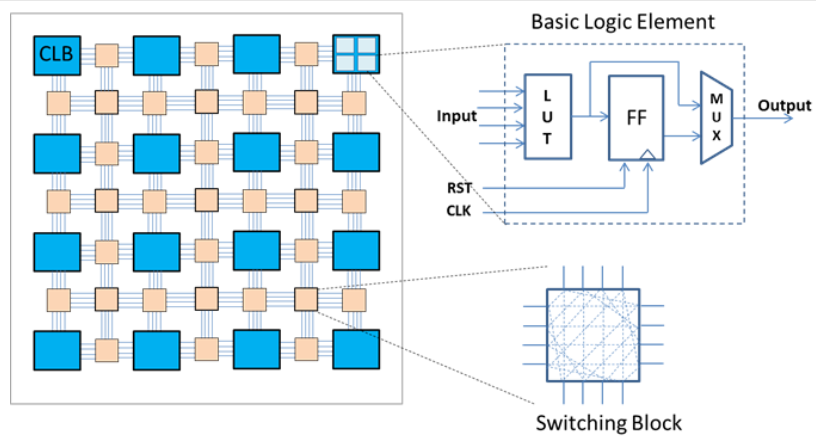
\includegraphics[width=0.7\textwidth]{img/ex_fpga.png}
    \caption{Abstract FPGA layout\cite{abs_fpga}}
    \label{fig:abs_fpga}
\end{figure}

\subsection{Flexible logic blocks}
Flexible logic blocks are what allow FPGAs to implement arbitrary logic functions. These consist of look-up tables, multiplexers, flip-flops and some small arithmetic logic, such as a 4-bit adder.

\begin{description}
    \item[LUT] An n-input look-up table is a 2\textsuperscript{n} bit memory which can be used to store the truth table for an n-input logic function, thereby functioning as a combinational logic gate(s).
    \item[Multiplexer] Multiplexers can be used to switch the output between the LUTs, flip-flops and arithmetic logic.
    \item[Flip-flops] Used together with the LUTs to implement clocked logic functions.
    \item[Arithmetic logic] Dependant on the FPGA, typically shared between a few logic blocks.
\end{description}

LUTs in modern FPGAs are typically around 6-inputs and so can store 64 combinations. For logic functions with more inputs than a single LUT, multiple LUTs can be combined and implement complex functions.

\subsection{Flexible routing}
FPGAs need to be able to connect different resources inside the chip to create the correct datapaths. This is achieved using large grids of wires between groups of logic blocks (sometimes called slices). The grids connect at switch boxes, which connects tracks to create data pathways between components. Latency in the signals sent are increased as the length of wire and amount of switch boxes increases, so minimising this is an important part of the process when a design is being mapped to an FPGA.

\subsection{Flexible IO}
FPGAs often have IO pins connected to logic that allows them to be programmed, implementing different IO protocols as required.

\subsection{Hard modules}
While flexible logic can be used to implement any logic function, the FPGA implementation will be slower than a dedicated hardware module. To increase performance in FPGAs, hard modules are embedded in the flexible logic to increase the performance when doing common tasks, like integer arithmetic or signal processing. 

Memory is often added to increase performance when large amounts of data must be stored and processed by the FPGA, as well as reduce the amount of LUTs used as data storage instead of logic functions. Block RAMs are embedded inside the flexible logic to reduce the physical distance between them, decreasing latency and increasing potential clock speed. As well as BRAMs, FIFOs and IO buffers are commonly used.

DSP (Digital Signal Processing) blocks are also embedded within the flexible logic blocks. These contain hardwired ALUs, and increase FPGA performance of arithmetic based tasks.

\subsection{FPGA programming and HDLs}
FPGAs implement logic defined by an HDL (Hardware Description Language). HDLs are similar to conventional coding languages in how they are written, but describe the structure and behaviour of a digital circuit at RTL (Register Transfer Level). There are also differences in the "compilation" of an HDL. Instead of being reduced to bytecode specific to an ISA, the HDL goes through the process of synthesis, where the formal definition is simplified into a design in terms of logic gates. The generated design is a netlist, effectively a list of the logic gates and the connections between them. The next stage in the process is place and route, which is specific to the FPGA being used. The netlist is mapped to resources inside the FPGA, such as LUTs and DSPs, with wires then routed between the resources to make the desired data paths. This stage requires optimisation, as the placement of the resources affects the distance of wire and latency, so changing the placement can result in better (or worse) maximum clock speeds and signal integrity. The result of place and route is a final design that can be implemented on an FPGA by generating a bitstream, a file that is loaded by the FPGA and configures the resources and switchboxes to implement the design.

\begin{figure}[H]
    \centering
    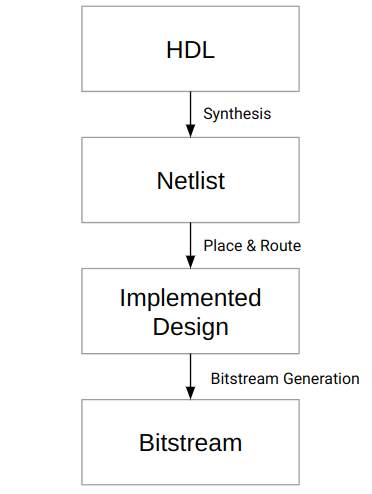
\includegraphics[width=0.5\textwidth]{img/fpga_synthesis_impl.png}
    \caption{FPGA design flow}
    \label{fig:fpga_design_flow}
\end{figure}

\section{Related work}
To the best of our knowledge, there are no existing works evaluating heterogeneous multicore RISC-V systems where all CPUs are peers and used for general-purpose computing, as described in \ref{sec:het_designs}. This project, therefore, represents novel research into this domain. There has been some research focussed on accelerator RISC-V heterogeneous designs, where a RISC-V host core(s) is used to control accelerator(s) comprised of specialised cores, RISC-V and otherwise. We've analysed some of these works for comparison against this project, and to learn how we may be able to achieve some of our objectives.

\subsection{A RISC-V Heterogeneous SoC for Embedded Devices\cite{valenterisc}}
This project is ongoing, and presents work designing a RV64 (RISC-V 64-bit) host core that offloads tasks to a programmable many-core accelerator (PMCA) made from RV32 cores, which implement extensions for machine learning and discrete signal processing. The suggested use-case for the SoC is in IoT applications and programmable embedded devices. The host core is Linux compatible, and offers a full OS that acts as a platform for programs that run on the PMCA. The use of a large RV64 core to allow a full Linux OS to run on the SoC provides a huge amount of flexibility to the programmer, as the OS implements features like CLI, memory virtualisation, networking and more that allow programs to be written much more generally than embedded software running without an OS. However, this usage of a full Linux OS could be considered excessive for the use-case as an embedded system. An embedded Linux OS would have a lower overhead due to the reduced services it offers, which is very beneficial in an embedded environment where efficiency is highly important. Unfortunately, no data is provided about the processing power or energy usage of the design.

\subsection{Muntjac multicore RV64 processor\cite{UCAM-CL-TR-972}}
Muntjac is an SoC generator comprising of multiple components, that can be used to produce a Linux capable SoC. There is only one type of core in the system, RV64, but the SoC can be multicore. The project report is dedicated to the design of the core and cache as opposed to usage in any devices, as the purpose is to provide an easily understood and extensible platform for specialised designs. This is excellently done - the project is very well presented and uses multiple open-standards like TileLink\cite{tilelink} to increase the ease of working with it. It would be possible for this project to be extended for a heterogeneous SoC design, but it appears that this has not yet been done in any public works that extend the project.

\subsection{HEROv2: Full-Stack Open-Source Research Platform for Heterogeneous Computing\cite{herov2}}
HEROv2 is an FPGA-based research platform for design and experimentation of heterogeneous systems. The platform consists of clustered RV32 cores as a PMCA and a host 64-bit ARMv8 or RV64 core. The host is single-core and the RISC-V core used is the CVA6\cite{zaruba2019cost} CPU, implementing the RV64IMAC ISA with M, S and U privilege levels for use with Unix-like operating systems. The platform includes a heterogeneous compiler for the system, allowing programs not written to explicitly leverage the accelerators to still make use of them. While also heterogeneous, this work uses the term in the host + accelerator form, instead of differing general-purpose CPUs both used as hosts. By basing the platform on FPGAs, HEROv2 allows researchers to modify the PMCA to meet their specific target application. The flexibility this brings makes the platform an ideal choice for rapid development and research of heterogeneous computing systems.

\subsection{JuxtaPiton: Enabling Heterogeneous-ISA Research with RISC-V and SPARC FPGA Soft-cores\cite{lim2018juxtapiton}}
JuxtaPiton is an open-source general-purpose heterogeneous processor developed by integrating a PicoRV32\cite{picorv32} core into the OpenPiton\cite{openpiton} research framework. OpenPiton uses a modified OpenSPARC T1 core, a completely different ISA to RISC-V. JuxtaPiton attempts to achieve greater efficiency by allowing the OpenSPARC core to assign processes to the PicoRV32 core. By offloading low intensity tasks to the PicoRV32 core when there are no others, the energy efficiency of the system is expected to be increased. The JuxtaPiton platform can run Debian Linux, keeping all features that OpenPuton has. The paper discusses the performance and area differences between the cores: the PicoRV32 had below 25\% of the performance of the OpenSPARC core, while using 23\% of the area. The paper does not attempt to measure the performance/power of the system, instead focussing on area. Overall JuxtaPiton is the most similar work to the aims of this project, and achieves extremely good results while providing a future platform for further heterogeneous research, suggesting that the PicoRV32 core could be swapped for any other RISC-V core.